\chapter{Software Containers}
\label{ch:containers}

\section{Software Containers}

\begin{wrapfigure}{l}{0.3\textwidth}
    \centering
    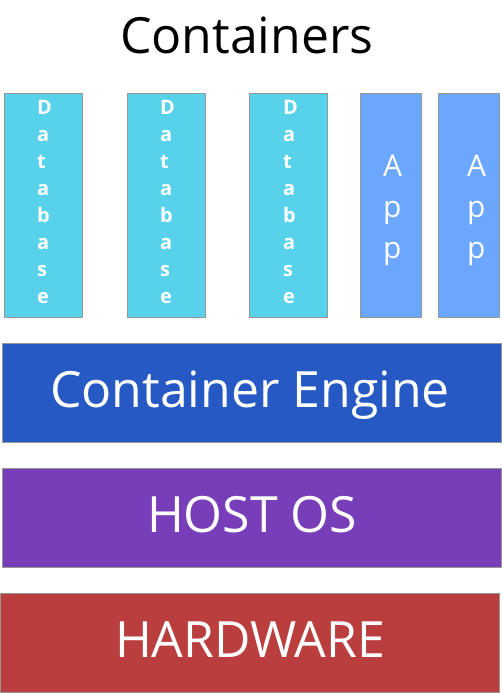
\includegraphics[width=3cm]{img/container}
    \caption{structuur van containers}
    \label{fig:containers}
\end{wrapfigure}

Software containers bestaan al een ruime tijd. In \cite{soltesz_container-based_2007} werd al gekeken naar de voordelen van software containers ten opzichte van hypervisors. Chroot (\cite{_linux_????}) is een concept dat veel deelt met software containers. Chroot zal de root directory van het huidige proces en zijn children veranderen. Er wordt een virtuele kopie gemaakt van het systeem waarin het proces kan werken. Het proces is dus afgesloten van het systeem en dit zorgt voor meer veiligheid bij het uitvoeren van processen.

Linux Containers of LXC (\cite{containers_linux_????}) is een implementatie van besturingssysteem virtualisatie. LXC kan meerdere geïsoleerde Linux systemen laten werken op één host. Deze geïsoleerde Linux systemen worden software containers genoemd. Deze containers worden ook getoond in figuur \ref{fig:containers} waarbij de apps en databases containers zijn.

Zoals al gezien is, is de rol van de hypervisor het delen en beheren van de middelen. Om containers te gebruiken, moet een ander deel de rol van de hypervisor overnemen. Cgroups is een Linux kernel extension die deze rol overneemt. Door middel van cgroups kunnen middelen worden beheerd voor processen. Het toont ook de mogelijkheden om backups te creëren van processen.

Eerder werd ook al aangehaald dat de processen van elkaar gescheiden moeten worden. Dit wordt bereikt door namespaces. De functies die name spaces voorzien zijn uitgebreid. Elke namespace heeft zijn eigen bestandssysteem structuur, netwerk interfaces en proces ID space. De containers delen de kernel met alle andere processen die op de kernel aan het werken zijn.

De containers zijn van elkaar afgesloten. Wanneer één container aangetast wordt, dan heeft dit geen rechtstreeks gevolg op de andere containers.

Toch zijn er een paar andere problemen zoals aangehaald in \cite{madhavapeddy_jitsu:_2015}. Processen die als root werken kunnen niet geïsoleerd worden van elkaar. Verder wordt er ook aangehaald dat strengere isolatie nodig is. (tabel 2, \cite{madhavapeddy_jitsu:_2015})

\section{Docker}

Docker (\cite{docker_docker_2016}) is een open source project om software containers te gebruiken voor programma's gemakkelijk te ontwikkelen en te laten werken op verschillende besturingssystemen.

Er zijn andere formaten zoals rkt \cite{_rkt_????} die het ook mogelijk maken om gemakkelijk software containers te gebruiken.

In 2015 werd het Open Container Initiative opgericht. Veel grote spelers op vlak van software containers zoals Docker, CoreOS, Microsoft en Google maken hier deel van uit. Samen willen ze een standaard voor software containers vastleggen. \cite{}.

De problemen die we bij software containers tegenkomen hebben voornamelijk betrekking tot beveiliging. Unikernels kunnen een veiliger alternatief zijn. In het volgende hoofdstuk worden de werking en mogelijkheden met unikernels bekeken.
